\documentclass[12pt]{article}

\usepackage{amsmath}
\usepackage{graphicx}
\usepackage[
  backend=biber,
  style=numeric-comp,
  sorting=none,
  maxcitenames=2,
  mincitenames=1
]{biblatex}



\addbibresource{refs/304IASCC.bib}

\title{
A Mechanistic Model for Radiation-Induced Segregation Controlled
Grain-Boundary Oxidation in Austenitic Stainless Steels
}

\author{Zhuo Wang \and Md Shahrier Hasan \and Jaime Marian}
\date{\today}

% \setlength{\parindent}{0pt}
% \setlength{\parskip}{0.8em}

\newcommand{\Vac}{\mathrm{V}}          % vacancy
\newcommand{\Int}{\mathrm{I}}          % self-interstitial
\newcommand{\GB}{\mathrm{GB}}
\newcommand{\eff}{\mathrm{eff}}
\newcommand{\intf}{\mathrm{int}}       % interface
\newcommand{\thr}{\mathrm{th}}         % threshold
\newcommand{\lat}{\mathrm{lat}}
\newcommand{\ox}{\mathrm{ox}}
\newcommand{\Ox}{\mathrm{O}}           % oxygen
\newcommand{\textciteyear}[1]{\citeauthor{#1} (\citeyear{#1})~\cite{#1}}



\usepackage{graphicx}
\usepackage{subcaption}
\graphicspath{{figures/}{../figures/}}

\usepackage{siunitx}
\usepackage{mhchem}

\DeclareSIUnit{\dpa}{dpa}
\DeclareSIUnit{\atpct}{at.\%}



\begin{document}

\maketitle


% ============================================================
\section{Introduction}
\label{sec:introduction}

\begin{figure}[htbp]\centering
\makebox[\textwidth][c]{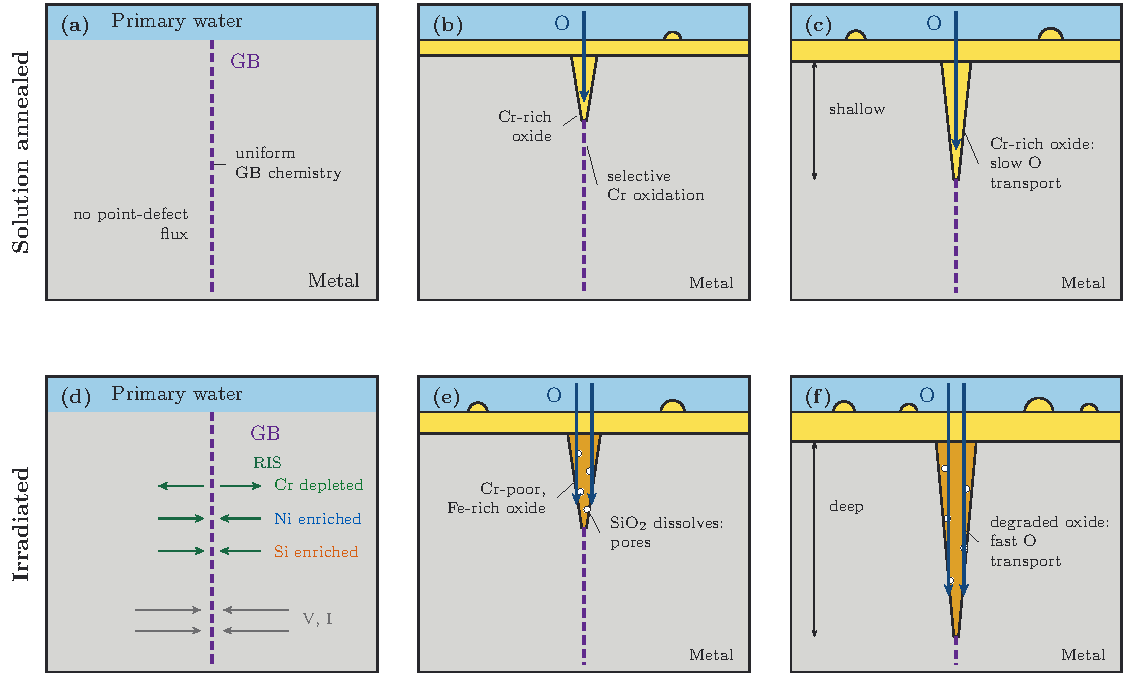
\includegraphics[width=18.6cm]{physical_picture}}
\caption{Physical picture of intergranular oxidation in primary water without
(a--c) and with (d--f) prior irradiation. (a) Solution-annealed boundary with
uniform chemistry. (b) Oxygen entering at the boundary mouth oxidizes Cr
selectively and forms a Cr-rich intergranular oxide. (c) The Cr-rich oxide
limits oxygen transport along the boundary and the penetration stays shallow.
(d) Irradiation drives point defects to the boundary and the resulting
radiation-induced segregation depletes Cr and enriches Ni and Si. (e) On
exposure the Cr-depleted boundary forms a Cr-poor, Fe-rich oxide, and the
segregated Si oxidizes and dissolves, leaving pores. (f) The degraded oxide
transports oxygen faster along the boundary and the oxide penetrates deeper.}
\label{fig:physical-picture}
\end{figure}

% ---- 1. Phenomenon, why it matters, key observations, question ----
Irradiation-assisted stress corrosion cracking (IASCC) is a major
degradation mode of austenitic stainless steel core internals in
light-water reactors \parencite{was2011irradiationassisted}. In irradiated
stainless steels exposed to high-temperature water, intergranularoxidation weakens grain boundaries and precedes intergranular crack initiation
\cite{was2024how}, and grain-boundary oxidation has been identified as
a necessary precursor of IASCC at low doses \cite{kuang2022highresolution}. In 304
stainless steel (304SS) exposed to pressurized water reactor (PWR) primary
water, the extent of this oxidation depends on the chemical changes
introduced by prior irradiation.
\textcite{deng2017effect} found that increasing the proton irradiation dose
produced deeper intergranular oxidation in 304 nuclear-grade stainless
steel after water exposure, accompanied by a decrease in the Cr content of
the intergranular oxide. Cr depletion is not the only chemical change that
matters. Using model alloys with Si and Cr contents chosen to mimic the
segregated boundary, \textcite{du2026silicon} showed that Si enrichment
promotes intergranular oxidation and cracking even when Cr is not
depleted: Si forms \ce{SiO2} that is unstable in high-temperature water
and dissolves preferentially, leaving a porous oxide that provides
pathways for oxygen diffusion along grain boundaries. These observations
connect irradiation to both the chemistry and the penetration depth of the
intergranular oxide. Turning them into a predictive relationship requires a
description of how the changing oxide composition and structure affect
oxygen transport and, consequently, the advance of the oxidation front.

% ---- 2. RIS sets the boundary composition; oxide Cr sets transport resistance ----
Radiation-induced segregation (RIS) establishes the local alloy
composition from which the intergranular oxide develops. Coupling between
solute and irradiation-generated point-defect fluxes redistributes
alloying elements near grain boundaries. Measurements on irradiated
304 nuclear-grade stainless steel reveal Cr depletion and Ni and Si enrichment
at the grain boundary \cite{deng2021grain}. Subsequent
oxidation selectively consumes alloying elements, changing both the oxide
composition and the adjacent metal, where Ni enrichment has also been
observed \cite{deng2021grain}. The lower Cr content of the oxide
formed on irradiated boundaries has been associated with reduced
resistance to oxygen diffusion \cite{deng2017effect}. 

% ---- 3. Si oxidation and dissolution add free volume to the same transport quantity ----
Si oxidation and dissolution alter this transport resistance by changing
the structure through which oxygen moves. The role of Si identified by
\textcite{du2026silicon} established with model alloys of systematically
varied Cr and Si contents in hydrogenated water, which allowed the
contributions of Cr depletion and Si enrichment to be separated. They
attributed the greater oxide degradation and cracking susceptibility at
higher Si content to dissolution of \ce{SiO2} in the inner oxide and the
resulting porous, defective film, and their STEM analysis of intergranular
oxides indicated faster grain-boundary diffusion at higher Si content. Related microscopy on
proton-irradiated 316L identified Si enrichment at oxide tips and
porosity behind them, consistent with preferential Si oxidation followed
by dissolution \cite{kuang2022highresolution}. Although 316L differs from 304SS in
bulk composition, this observation is used here as mechanistic support
rather than as a quantitative reference; the same oxidation and
dissolution of segregated Si appears as a step in the IASCC mechanism
summarized by \textcite{was2024how}. Together, these studies provide
a basis for including dissolution-generated free volume in the transport
description. With the dependence on Cr content, they motivate
representing the evolving oxide composition and free volume through a
single effective oxygen diffusivity, which connects the segregation of
multiple elements to a common quantity governing oxygen transport.

% ---- 4. Existing models and the gap ----
Each half of this sequence has been modeled separately, and the two
halves are not equally developed. The segregation half is settled enough
that the boundary composition can be computed rather than only measured.
Since the inverse-Kirkendall and rate-theory descriptions of RIS in
concentrated alloys \parencite{marwick1978segregation,wiedersich1979theory},
the composition profile at a grain boundary has been obtained from the
coupled fluxes of point defects and alloying elements, with Fe--Cr--Ni
parameterizations that reproduce the measured dose and temperature
dependence of Cr depletion and Ni enrichment
\parencite{allen1998modeling}. Current models go further and
resolve the sink itself, predicting segregation at grain boundaries and
dislocation cell walls \parencite{kadambi2025phasefield} and the
conditions under which Cr switches from enrichment to depletion
\parencite{oplinger2026radiationinduceda}. What all of these models return
is the segregation profile. None carries that profile into what the
boundary does next: the profile is an end point, not the initial
condition for a subsequent process.
% Keys not yet in the Zotero export (guessed in Better-BibTeX style; rename
% to match once added): marwick1978segregation, wiedersich1979theory.

On the oxidation side, the dependence of intergranular penetration depth
on dose and exposure time has been characterized
experimentally \parencite{deng2017effect,deng2020corrosion}, but existing
kinetic models of grain-boundary oxidation do not respond to the boundary
chemistry. Models that resolve oxygen transport along the boundary treat
the oxygen diffusivity as a single constant: in analytical or
semi-analytical solutions that give the penetration depth in closed form
\parencite{fisher1951calculation,xu2015modeling,evans2013mechanism}, in
finite-element descriptions in which it is fitted to measured oxide depths
through a parabolic law \parencite{zhao2011modeling,karabela2013oxygen} or
prescribed together with a constant reaction rate
\parencite{aoyagi2012crystal}, and in phase-field simulations of a single
stoichiometric chromia intrusion
\parencite{derancourt2015modelling,rancourt2025viscoplasticity}. In none of
these does the diffusivity depend on the composition of the oxide that has
formed. Where the oxide identity does control transport, in multilayer
descriptions of planar scales \parencite{harrison1984ratios,huang2022multilayer}
and in the mechanistic treatment of uniform corrosion in high-temperature
water \parencite{robertson1991mechanism}, the controlling phase is fixed at
the outset rather than selected by the local alloy composition. The
boundary composition enters only after conversion into an empirical
parameter, as a Cr-content-dependent dissolution rate in sensitized steels
\parencite{osawa1985computer} or as a sensitization index that increases
with neutron fluence in the slip-oxidation prediction of crack growth
\parencite{ford1996quantitative}; crack-growth models that require a
grain-boundary oxidation law borrow rate constants measured on bulk
surfaces \parencite{shoji2010formulating}. Thermodynamic selection of the
oxide phases from the local alloy composition has been implemented for a
Ni-base superalloy \parencite{fang2022numerical}, but with a constant
oxygen diffusivity, the bulk composition at the boundary, and without the
Cr oxide that limits transport. No model takes the irradiation-modified
boundary composition as input and lets the resulting oxide composition set
the oxygen transport that governs further penetration.

To our knowledge, no model connects the segregated composition to the
advance of the oxidation front through a transport quantity computed from
both. Establishing this connection requires tracking how the segregated
alloy supplies the interfacial reactions, how those reactions change the
oxide, and how the resulting diffusivity affects subsequent oxygen
delivery. Segregation profiles, oxide composition, interfacial Ni
enrichment, and penetration depth then provide complementary observables
for assessing the coupling.

% ---- 5. This work ----
Here, we develop a coupled RIS and grain-boundary oxidation model for
304SS, represented by the Fe--Cr--Ni--Si system. The model links
defect-mediated solute redistribution and selective interfacial
consumption to an effective oxygen diffusivity, \(D_{\mathrm{eff}}\),
determined by the evolving oxide composition and free volume. Within
this description, increasing the Cr content of the oxide lowers the
effective diffusivity, whereas Si oxidation followed by complete
dissolution contributes free volume that enhances transport. The same
\(D_{\mathrm{eff}}\) enters both oxygen transport along the grain boundary
and oxygen delivery across the oxide to the metal interface. The model
therefore connects RIS to oxidation kinetics through the resulting change
in oxygen transport, with metal consumption feeding back on the local
composition. The complete-dissolution treatment is a simplification
motivated by the mechanism discussed by Du and co-workers
\cite{du2026silicon}. We examine the dose and exposure-time dependence of
oxide penetration under sequential irradiation and water exposure, using
separate calibration of the RIS and oxidation components and a common
set of oxidation parameters across doses. The framework also permits
predictions of concurrent RIS and oxidation within the same transport
description.

\printbibliography
\end{document}
